\documentclass{article}
\usepackage{hw_style}
\usepackage{enumerate}
\usepackage{graphicx}
\usepackage{verbatim}

% Homework Specific Information
\newcommand{\hmwkTitle}{Homework \#3}
\newcommand{\hmwkDueDate}{ September 16, by 3:00 p.m.}
\newcommand{\hmwkAuthorName}{Kurt Rudolph}%Name:
\newcommand{\hmwkNetID}{rudolph9}%your netid
\newcommand{\hmwkNotes}{}%I worked with...

\newcommand{\hmwkSubTitle}{}
\newcommand{\hmwkClass}{STAT 400}
\newcommand{\hmwkClassTime}{}
\newcommand{\hmwkClassInstructor}{Yinxiao Huang}

\begin{document}
\begin{spacing}{1.1}
\maketitle
%=============================Problem1=========================%
\newpage
\begin{homeworkProblem}
		Homer Simpson is going to Moe's Bar for some \emph{Flaming Moe's}.  Let $X$ denote the number of \emph{Flaming Moe's} that Homer Simpson will drink.  Suppose $X$ has the following probability distribution: 
	\\ 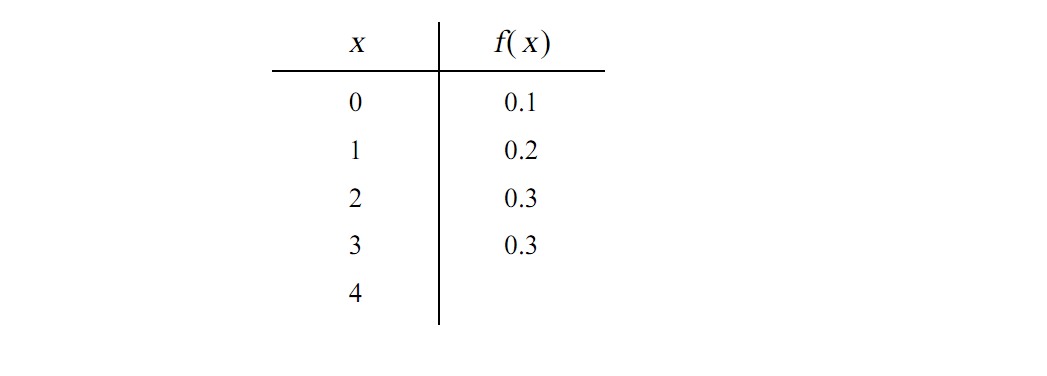
\includegraphics[width=\linewidth]{prob1.png}		
	\begin{enumerate}[(a)]
		\item Find the probability $F(4) = P(X = 4)$
			\begin{homeworkSection}{Solution}
				\[P(X = 4) = 1 - \left( {0.1 + 0.2 + 0.3 + 0.3} \right) = 0.1\]
			\end{homeworkSection}
		\item Find the probability $P(X \ge 1)$
			\begin{homeworkSection}{Solution}
				\[P\left( {X \ge 1} \right) = 1 - 0.1 = 0.9\]
			\end{homeworkSection}
		\item Compute the probability $P(X \ge 1 | X < 3)$
			\begin{homeworkSection}{Solution}
				\[P\left( {X \geqslant 1|X < 3} \right) = \frac{{P\left( {X \geqslant 1 \cap X < 3} \right)}}{{P\left( {X < 3} \right)}} = \frac{{0.5}}{{0.6}} = 0.83\]
			\end{homeworkSection}
		\item Compute the expected value of $X, E(X)$
			\begin{homeworkSection}{Solution}
				\[E\left[ X \right] = 0(0.1) + 1(0.2) + 2(0.3) + 3(0.3) + 4(0.1) = 2.1\]
			\end{homeworkSection}
		\item Compute the standard deviation of $X$, $SD(X)$
			\begin{homeworkSection}{Solution}
\[\begin{gathered}
  \sigma  = \sqrt {{{\left( {0(0.1) - 2.1} \right)}^2} + {{\left( {1(0.2) - 2.1} \right)}^2} + {{\left( {2(0.3) - 2.1} \right)}^2} + {{\left( {3(0.3) - 2.1} \right)}^2} + {{\left( {4(0.1) - 2.1} \right)}^2}}  \hfill \\
   = \sqrt {4.41 + 3.61 + 2.25 + 1.44 + 2.89}  = 3.82 \hfill \\ 
\end{gathered} \]
			\end{homeworkSection}
	Suppose each \emph{Flaming Moe} costs \$1.50, and there is a cover charge of \$1.00 at the door.  Let $Y$ denote the amount of money Homer Simpson spends at the bar Then $Y = 1.50 \cdot X+1.00$.
		\item Find the probability that Homer would spend over \$5.00.
			\begin{homeworkSection}{Solution}
				\[P(Y>\$5.00) = P(X \ge 3) = 0.3 +0.1 = 0.4\]
			\end{homeworkSection}
		\item  Find the expected amount of money that Homer Simpson would spend, $E(Y)$.
			\begin{homeworkSection}{Solution}
				\[ E[Y] = 1.5 E[X]+1 = \$4.15 \]
			\end{homeworkSection}
		\item  Find the standard deviation for the amount of money that Homer Simpson would spend, $SD(Y)$.
			\begin{homeworkSection}{Solution}
				\[ SD(Y) = 1.5SD(X) = 5.73 \]
			\end{homeworkSection}
	\end{enumerate}
\end{homeworkProblem}
%=============================Problem2==========================%	
\begin{homeworkProblem}
	Suppose that probability that a duck hunter will successfully hit a duck is 0.40 on any given shot.  Suppose also that the outcome of each shot is independent from the others.  
	\begin{enumerate}[(a)]
		\item What is the probability that the first successful hit will be on the fourth shot?
			\begin{homeworkSection}{Solution}
				\[(0.6)(0.6)(0.6)(0.4) = 0.08\]
			\end{homeworkSection}
		\item What is the probability that the first successful hit will be on the ninth shot?
			\begin{homeworkSection}{Solution}
				\[{(0.6)^8}(0.4) = 0.006\]
			\end{homeworkSection}
		\item What is the probability that the hunter would have three successful hits in nine shots?
			\begin{homeworkSection}{Solution}
				\[{(0.6)^6}{(0.4)^3} = 0.003\]
			\end{homeworkSection}
		\item What is the probability that the hunter would have at least six successful hits in nine shots?
			\begin{homeworkSection}{Solution}
				
			\end{homeworkSection}
	\end{enumerate}
\end{homeworkProblem}
%=============================Problem3==========================%	
\begin{homeworkProblem}
	An advertising company has 7 men and 5 women.  Suppose the company has to select a team of 4 members to work on the new hybrid car, Hyper Geo Metro 2011 : ), commercial.  
	\begin{enumerate}[(a)]
		\item If the members of the team are selected at random, what is the probability that 2 men and 2 women will be selected?
			\begin{homeworkSection}{Solution}
		
			\end{homeworkSection}
		\item What is the probability that men will constitute a majority in the team?
			\begin{homeworkSection}{Solution}
		
			\end{homeworkSection}			
	\end{enumerate}
\end{homeworkProblem}
%=============================Problem4==========================%	
\begin{homeworkProblem}
	Suppose Homer Simpson has five coins: 2 nickels, 2 dimes and 1 quarter.  Let $X$ denote the amount Bart gets if he steals two coins at random.  
	\begin{enumerate}[(a)]
		\item  Construct the probability distribution of $X$.
			\begin{homeworkSection}{Solution}
		
			\end{homeworkSection}
		\item  Find the expected value of the amount that Bart gets, $E(X)$.
			\begin{homeworkSection}{Solution}
		
			\end{homeworkSection}
		\item  Find the standard deviation $SD(X)$.
			\begin{homeworkSection}{Solution}
		
			\end{homeworkSection}
	\end{enumerate}
\end{homeworkProblem}
%=============================Problem5==========================%	
\begin{homeworkProblem}
	Tom works the night shift at a gas station on the edge of champaign.  From past experience, Tom know that 40\% of all customers who purchase gas pay at the pump with a credit card.  Assume that customers either pay at the pump with a credit card or not independently of each other. 
	\begin{enumerate}[(a)]
		\item Out of 15 customers who purchase gas, how many would you expect to pay at the pump with a credit card?
			\begin{homeworkSection}{Solution}
		
			\end{homeworkSection}
		\item What is the probability that exactly 5 customers out of 15 pay at the pump with a credit card?
			\begin{homeworkSection}{Solution}
		
			\end{homeworkSection}
		\item  What is the probability that at least 4 customers out of 15 pay at the pump with a credit card?
			\begin{homeworkSection}{Solution}
		
			\end{homeworkSection}
		\item What is the probability that the fourth customer purchasing gas is the first one to pay at the pump with a credit card?
			\begin{homeworkSection}{Solution}
		
			\end{homeworkSection}
		\item What is the probability that the fourth customer to pay at the pump with a credit card is the fifteenth customer purchasing gas?
			\begin{homeworkSection}{Solution}
		
			\end{homeworkSection}	
		\item What is the probability that the twentieth customer purchasing gas is the sixth one to pay at the pump with a credit card?		
			\begin{homeworkSection}{Solution}
		
			\end{homeworkSection}	
	\end{enumerate}
\end{homeworkProblem}
%=============================Problem6==========================%	
\begin{homeworkProblem}
	Tom works the night shift at a gas station on the edge of Champaign. One night he mixed 3 stale doughnuts in with 12 fresh doughnuts. That night 6 customers bought one doughnut each, selecting them at random. What is the probability that at least 2 stale doughnuts were sold?
	\begin{homeworkSection}{Solution}
		
	\end{homeworkSection}
\end{homeworkProblem}
%=============================Problem7==========================%	
\begin{homeworkProblem}
	A customer for a home insurance policy owns a \$200,000 home. The probability is 0.1\% that the home will be totally destroyed by fire, and the probability is 0.5\% that
the home will suffer a 50\% loss due to fire. If we ignore all other partial losses, what premium should the insurance company charge for a policy just to break even?
	\begin{homeworkSection}{Solution}
		
	\end{homeworkSection}
\end{homeworkProblem}
%=============================Problem8==========================%	
\begin{homeworkProblem}
	A box contains 2 green and 3 red marbles. A person draws a marble from the box at random {\bf without replacement}. If the marble drawn is red, the game stops. If it is green, the person draws again until the red marble is drawn (note that total number of marbles drawn cannot exceed 3 since there are only 2 green marbles in the box at the start). Let the random variable $X$ denote the number of {\bf green} marbles drawn.
	\begin{enumerate}[(a)]
		\item Find the probability distribution of $X$. [ Hint: There are only 3 possible outcomes for this experiment. It would be helpful to list these three outcomes ( three possible sequences of colors of marbles drawn ). It may be helpful to make a tree diagram for this experiment. Remember that all ( three ) probabilities must add up to one. ]
			\begin{homeworkSection}{Solution}
		
			\end{homeworkSection}
		\item Suppose it costs \$5 to play the game, and the person gets \$10 for each green marble
drawn. Is the game fair * ? Explain. [ Hint: Find  $\mu_X = E(X)$, the average (expected) number of green marbles drawn per game. ]
	\end{enumerate}
\end{homeworkProblem}
%=============================Problem9==========================%	
\begin{homeworkProblem}
	{\bf 2.2-2}	Let the random variable $X$ have the p.m.f. 
	\[f\left( x \right) = \frac{{{{\left( {\left| x \right| + 1} \right)}^2}}}{9},x =  - 1,0,1\]
	Compute $E(X),E(X^2)$, and $E(3X^2 - 2X +4)$.
	\begin{homeworkSection}{Solution}
		\[\begin{gathered}
  E\left( X \right) = \left( { - 1} \right)\left( {\frac{4}{9}} \right) + \left( 0 \right)\left( {\frac{1}{9}} \right) + \left( 1 \right)\left( {\frac{4}{9}} \right) = 0 \hfill \\
  E\left( {{X^2}} \right) = {\left( { - 1} \right)^2}\left( {\frac{4}{9}} \right) + \left( 0 \right)\left( {\frac{1}{9}} \right) + {\left( 1 \right)^2}\left( {\frac{4}{9}} \right) \hfill \\
  E\left( {3{X^2} - 2X + 4} \right) = 3\left( {\frac{8}{9}} \right) - 2\left( 0 \right) + 4 = \frac{{20}}{3} \hfill \\ 
\end{gathered} \]
	\end{homeworkSection}
\end{homeworkProblem}
%=============================Problem10==========================%	
\begin{homeworkProblem}
	{\bf 2.2-4} In a state lottery, a three-digit integer is selected at random.  A player bets \$1 on a particular number, and if that number is selected, the payoff is \$500 minus the \$1 paid for the ticket.  Let $X$ equal the payoff to the bettor, namely, -\$1 or \$499, and find $E(X)$.  
	\begin{homeworkSection}{Solution}
		\[\$ 499\left( {\frac{1}{{1000}}} \right) - \$ 1\left( {\frac{{999}}{{1000}}} \right) =  - \$ 0.50\]
	\end{homeworkSection}
\end{homeworkProblem}
%=============================Problem11==========================%	
\begin{homeworkProblem}
	{\bf 2.2-8}	Let the p.m.f. of $X$ be defined by $f(x) = 6/(\pi^2 x^2), x = 1, 2, 3, \dots$ Show that $E(X)$ does not exist in this case.  (Can you show that $f(x)$ is a p.m.f?)
	\begin{homeworkSection}{Solution}
		\[\begin{gathered}
  \sum\limits_{x = 1}^\infty  {\frac{6}{{{\pi ^2}{x^2}}}}  = \frac{6}{{{\pi ^2}}}\sum\limits_{x = 1}^\infty  {\frac{1}{{{x^2}}}}  = \frac{6}{{{\pi ^2}}}\frac{{{\pi ^2}}}{6} \Rightarrow p.d.f \hfill \\
  E\left( X \right) = \sum\limits_{x = 1}^\infty  {x\frac{6}{{{\pi ^2}{x^2}}}}  = \frac{6}{{{\pi ^2}}}\sum\limits_{x = 1}^\infty  {\frac{1}{x}}  = \infty  \hfill \\ 
\end{gathered} \]
		Hence $E(X)$ does not exist.
	\end{homeworkSection}
\end{homeworkProblem}
%=============================Problem12==========================%	
\begin{homeworkProblem}
	{\bf 2.3-4}	 Let $\mu$ and $\sigma^2$ denote the mean and variable of the random variable $X$.  Determine $E[(X - \mu)/ \sigma$ and $E\{[ (X - mu)/\sigma]^2\}$.  
	\begin{homeworkSection}{Solution}
		\[\begin{gathered}
  E\left[ {\frac{{X - \mu }}{\sigma }} \right] = \left( {\frac{1}{\sigma }} \right)\left[ {E\left( X \right) - \mu } \right] = \left( {\frac{1}{\sigma }} \right)\left( {\mu  - \mu } \right) = 0 \hfill \\
  E\left[ {{{\left( {\frac{{X - \mu }}{\sigma }} \right)}^2}} \right] = \left( {\frac{1}{{{\sigma ^2}}}} \right)E\left[ {{{\left( {X - u} \right)}^2}} \right] = \left( {\frac{1}{{{\sigma ^2}}}} \right)\left( {{\sigma ^2}} \right) = 1 \hfill \\ 
\end{gathered} \]
	\end{homeworkSection}
\end{homeworkProblem}


\begin{comment}%==========================================================
%=============================Problemi==========================%	
\begin{homeworkProblem}
	
	\begin{homeworkSection}{Solution}
		
	\end{homeworkSection}
\end{homeworkProblem}
%=============================Problemi==========================%	
\begin{homeworkProblem}
	
	\begin{enumerate}[(a)]
		\item 
			\begin{homeworkSection}{Solution}
		
			\end{homeworkSection}
	\end{enumerate}
\end{homeworkProblem}
%=============================Problemi==========================%	
\begin{homeworkProblem}
	{\bf }	
	\begin{homeworkSection}{Solution}
		
	\end{homeworkSection}
\end{homeworkProblem}
%=============================Problemi==========================%	
\newpage
\begin{homeworkProblem}
	{\bf  }	
	\begin{enumerate}[(a)]
		\item 
			\begin{homeworkSection}{Solution}
		
			\end{homeworkSection}
	\end{enumerate}
\end{homeworkProblem}
%=============================Problemi=========================%
\newpage
\begin{homeworkProblem}
	
	\begin{homeworkSection}{Solution}
		
	\end{homeworkSection}
\end{homeworkProblem}

\end{comment}%=========================================================

	
\end{spacing}
\end{document}














